\documentclass{article}
\usepackage[a4paper, portrait, margin=1in]{geometry}
\usepackage{graphicx}
\usepackage{array}
\usepackage{listings}
\usepackage{xcolor}
\usepackage[utf8]{inputenc}
\usepackage{blindtext}
\usepackage[export]{adjustbox}
\usepackage{enumerate}
\usepackage{amsmath}
\usepackage[skip=0.5ex]{subcaption}
\usepackage{caption}
\usepackage{lipsum}
\usepackage{tabularx}
\usepackage{makecell}
\usepackage{subdepth}
\usepackage{cite}

\definecolor{codegreen}{rgb}{0,0.6,0}
\definecolor{codegray}{rgb}{0.5,0.5,0.5}
\definecolor{codepurple}{rgb}{0.58,0,0.82}
\definecolor{backcolour}{rgb}{0.95,0.95,0.92}

\newtheorem{theorem}{Theorem}

\lstdefinestyle{mystyle}{
    backgroundcolor=\color{backcolour},
    commentstyle=\color{codegreen},
    keywordstyle=\color{magenta},
    numberstyle=\tiny\color{codegray},
    stringstyle=\color{codepurple},
    breakatwhitespace=false,
    breaklines=true,
    captionpos=b,
    keepspaces=true,
    numbers=left,
    numbersep=5pt,
    showspaces=false,
    showstringspaces=false,
    showtabs=false,
    tabsize=4
}



\begin{document}

\title{Student Id: 9910821}
\date{}

\maketitle
\section*{Introduction}
This report is a two part study of:
\begin{enumerate}[I)]
  \item Pricing a convertible bond contract in  which, \textbf{at expiry} $T$ the  holder  has  the option to  choose  between  receiving the principle $F$ or alternatively receiving $R$ underlying stocks with price $S$
  \item An extension to the above contract where the holder is able to exercise the decision to convert the bond in stock at \textbf{any time before} the maturity of the contract. This is known as an American embedded option
\end{enumerate}
through the use of advanced numerical methods such as Crank-Nicolson with PSOR.

\section{European Option Convertible Bond}
The PDE describing such a convertible bond contract is given by
\begin{equation}
  \frac{\partial V}{\partial t} + \frac{1}{2}\sigma^{2}S^{2\beta}\frac{\partial^2 V}{\partial S^2}+\kappa(\theta (t) -S)\frac{\partial V}{\partial S} -rV + Ce^{-\alpha t} =0
  \label{eq:pde_convertible}
\end{equation}

To use advanced numerical methods of (approximately) solving such PDEs we need a numerical scheme. This is a method of rewriting Equation \ref{eq:pde_convertible} as a matrix equation as in Equation \ref{eq:matrix_convertible}.
\begin{equation}
\begin{pmatrix}
b_0 & c_0 & 0 & 0 & . & . & . & . & 0\\[6pt]
a_1 & b_1 & c_1 & 0 & . & . & . & . & .\\[6pt]
0 & a_2 & b_2 & c_2 & 0 & . & . & . & .\\[6pt]
. & . & . & . & . & . & . & . & .\\[6pt]
. & . & . & . & a_j & b_j & c_j & . & .\\[6pt]
. & . & . & . & . & . & . & . & .\\[6pt]
0 & . & . & . & . & . & . & a_{jmax} & b_{jmax}
\end{pmatrix}
\begin{pmatrix}
{V_j^0}\\[6pt]
{V_j^1}\\[6pt]
{V_j^2}\\[6pt]
.\\[6pt]
{V_j^i}\\[6pt]
.\\[6pt]
{V_{jmax}^i}
\end{pmatrix}
=
\begin{pmatrix}
{d_j^0}\\[6pt]
{d_j^1}\\[6pt]
{d_j^2}\\[6pt]
.\\[6pt]
{d_j^i}\\[6pt]
.\\[6pt]
{d_{jmax}^i}
\end{pmatrix}
  \label{eq:matrix_convertible}
\end{equation}
where $j$ represents the steps in $S$ and $i$ the steps in $t$. The Crank-Nicolson method takes approximations of derivatives by Taylor expanding at the half time steps thus yielding
\begin{equation}
  \frac{\partial V}{\partial t} \approx \frac{V_j^{i+1}-{V_j^i}}{\Delta t}
  \label{eq:dvdt}
\end{equation}
\begin{equation}
  \frac{\partial V}{\partial S} \approx \frac{1}{4 \Delta S}(V_{j+1}^{i}-{V_{j-1}^i}+V_{j+1}^{i+1}-V_{j-1}^{i+1})
  \label{eq:dvds}
\end{equation}
\begin{equation}
  \frac{\partial^2 V}{\partial S^2} \approx \frac{1}{2 \Delta S^2}(V_{j+1}^{i}-2{V_{j}^i}+V_{j+1}^{i+1}-2V_{j}^{i+1}+V_{j-1}^{i+1})
  \label{eq:d2vds2}
\end{equation}
\begin{equation}
  V \approx \frac{1}{2}(V_{j}^{i}+{V_{j}^{i+1}}).
  \label{eq:v}
\end{equation}
So substituting Equations \ref{eq:dvdt} - \ref{eq:v} into Equation \ref{eq:pde_convertible} gives the numerical scheme for the non-boundary regime $1 \leq j < jmax$ .
\begin{equation}
  a_j = \frac{\sigma^{2}S^{2\beta}}{4\Delta S^2} - \frac{\kappa(\theta-S)}{4 \Delta S}
  \label{eq:aj}
\end{equation}
\begin{equation}
  b_j = \frac{1}{\Delta t} - \frac{\sigma^2S^{2\beta}}{2 \Delta S^2} - \frac{r}{2}
  \label{eq:bj}
\end{equation}
\begin{equation}
  c_j =\frac{\sigma^{2}S^{2\beta}}{4\Delta S^2} + \frac{\kappa(\theta-S)}{4 \Delta S}
  \label{eq:cj}
\end{equation}
\begin{equation}
  d_j = -\frac{V_{j}^{i+1}}{\Delta t} - \frac{\sigma^2S^{2\beta}}{4 \Delta S^2}(V_{j+1}^{i+1}-2V_{j}^{i+1}+V_{j-1}^{i+1}) - \frac{\kappa(\theta-S)}{4\Delta S}(V_{j+1}^{i+1}-V_{j-1}^{i+1})+\frac{r}{2}V_j^{i+1}-Ce^{-\alpha t}
  \label{eq:dj}
\end{equation}
The boundary conditions are problem dependent so for this particular we have two boundaries at $S=0$ and \({\lim}_{S \to +\infty}\).
Consider the first boundary, when $S=0$ i.e $j=0$. Using Equations \ref{eq:dvdt} and \ref{eq:v} and a modified Equation \ref{eq:dvds} which becomes
\begin{equation}
  \frac{\partial V}{\partial S} \approx \frac{1}{\Delta S}(V_{j+1}^{i}-{V_{j}^i}).
  \label{eq:modified_dvds}
\end{equation}
The numerical scheme after substituing the approximated derivates is now given by
\begin{equation}
  a_0 = 0
  \label{eq:a0}
\end{equation}
\begin{equation}
  b_0 = -\frac{1}{\Delta t} - \frac{\kappa\theta}{\Delta S} - \frac{r}{2}
  \label{eq:b0}
\end{equation}
\begin{equation}
  c_0 =\frac{\kappa\theta}{\Delta S}
  \label{eq:c0}
\end{equation}
\begin{equation}
  d_0 = (-\frac{1}{\Delta t}+\frac{r}{2})V_{j}^{i+1}-Ce^{-\alpha t}
  \label{eq:d0}
\end{equation}
For the \({\lim}_{S \to +\infty}\) we have the condition that
\begin{equation}
  \frac{\partial V}{\partial t} +\kappa(X -S)\frac{\partial V}{\partial S} -rV + Ce^{-\alpha t} =0
  \label{eq:large_s_boundary}
\end{equation}
with the ansatz
\begin{equation}
  V(S,t)=SA(t)+B(t).
  \label{eq:ansatz}
\end{equation}
It can be shown (See Appendix 1) by partial differentiation and integrating using an integrating factor method that
\begin{equation}
  A(t)=Re^{(\kappa+r)(t-T)}
  \label{eq:A}
\end{equation}
and\begin{equation}
  B(t)=-XRe^{(\kappa+r)(t-T)}+\frac{C}{\alpha+r}e^{-\alpha t}-\frac{C}{\alpha+r}e^{-(\alpha+r)T+rt}+XRe^{r(t-T)}.
  \label{eq:B}
\end{equation}
Finally we have the last part of the numerical scheme as
\begin{equation}
  a_0 = 0
  \label{eq:amax}
\end{equation}
\begin{equation}
  b_0 = 1
  \label{eq:bmax}
\end{equation}
\begin{equation}
  c_0 =0
  \label{eq:cmax}
\end{equation}
\begin{equation}
  d_0 = SA(t)+B(t).
  \label{eq:dmax}
\end{equation}
Using this complete numerical scheme, the method is to solve backwards in time from $i=imax$ to $i=0$ where at each time step the Equation \ref{eq:matrix_convertible} is solved using
a method such as Successive Over Relaxation (SOR) for $j=0\to jmax$.
\par\noindent\rule{\textwidth}{0.4pt}
\subsection{Investigating $\beta$ and $\sigma$}
For the rest of this section assume these values were used unless otherwise specified:
$T=2$, $F=95$, $R=2$, $r=0.0229$, $\kappa=0.125$, $\mu=0.0113$, $X=47.66$, $C=1.09$, $\alpha=0.02$, $\beta=0.486$ and $\sigma=3.03$.
The value of the option $V(S,t)$ was investigated as a function of the initial underlying asset
price $S_0$ for two cases:
\begin{enumerate}[1)]
  \item ($\beta=1$, $\sigma=0.416$) with all other paramaters as previously defined
  \item ($\beta=0.486$, $\sigma=3.03$) with all other paramaters as previously defined
\end{enumerate}
The Crank-Nicolson method with the numerical scheme as calculated previously, combined with a SOR iterative method of solving the matrix equation, was implemented in code.
This produced the plots seen in Figure \ref{fig:varying_s}.
\clearpage
\begin{figure}[!th]
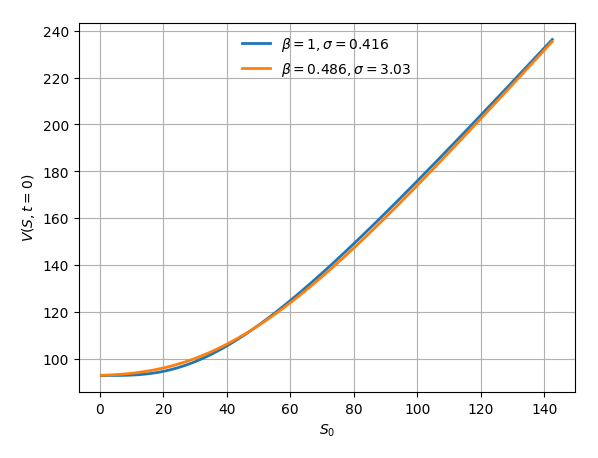
\includegraphics[width=0.65\textwidth,center]{../images/european_varying_s.png}
\caption{Value of the convertible bond $V(S,t=T)$ against inital underlying asset price at time $S_0$ for two combinations of $\beta$ and $\sigma$.}
\label{fig:varying_s}
\end{figure}
The two configurations were therefore found to have the same effect and produce plots for the price of the bond which were very close.
This prompted further analysis on the linked relationship between $\beta$, $\sigma$ and $V(S,t)$.
A 3D graph of the value of the portfolio for a particular $S_0$, here chosen to be equal to $X$, and the two other parameters was plotted.
Figure \ref{fig:3d_relationship} illustrates such a relationship which is interesting both in shape and in what it can be modelled by.
Going back a few steps, the risk-neutral process followed by the underlying stock price is given by
 \begin{equation}
  dS = \kappa ( \theta (t)-S)dt+\sigma S^{\beta}dW
  \label{eq:process}
\end{equation}
which is an Ornstein-Uhlenbeck (OU) process \cite{thierfelder2015trending} with a drift term of function $\theta(t)$ , together with a Constant Elasticity of Variance \cite{cev} model where the local variance is a powerlaw of elasticity.
Using this model, $\sigma$ is defined to be the actual Black-Scholes volatility or standard deviation of the underlying asset, while $\beta$ is the elasticity parameter of the local volatility.
\begin{figure}[!bh]
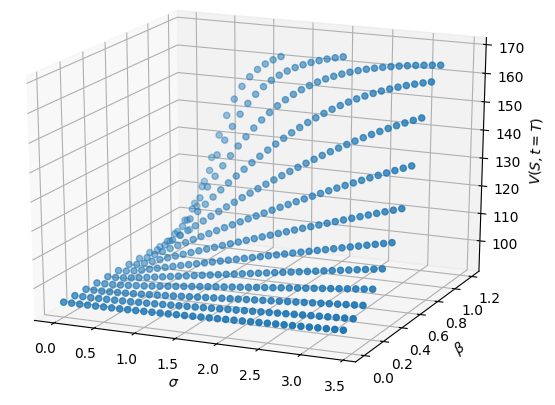
\includegraphics[width=0.65\textwidth,center]{../images/3d_european_varying_s_varying_sigma_varying_beta.png}
\caption{Value of the convertible bond $V(S=X,t=T)$ against parameters $\beta$ and $\sigma$.}
\label{fig:3d_relationship}
\end{figure}
Moreover, using this model the values of $\beta$ which should be used are for $\leq1$.
Above this, there are implications on the inaccessibility of the origin which for a stock price means it cannot go bankrupt which is not true.
Thus, we shall stick for values of $\beta\leq1$ here.
In this regime, the model captures the so-called 'leverage effect' which practically means that stock price and volatily are inversely proportional \cite{chan}.
The parameter $\beta$ in Equation \ref{eq:process} controls the steepness of the implied volatility skew which is something seen in Figure \ref{fig:3d_relationship}.
The parameter $\sigma$ is now part of a scale parameter which fixes the 'at-the-money' ($S$ close to $X$ regime) volatility level.
So, there are $\sigma-\beta$ planes on Figure \ref{fig:3d_relationship} which have close values of the convertible bond for multiple combinations of ($\sigma$ , $\beta$).
This happens since having a steep implied variance skew but a lower actual variation, which is an average of a time period, and the other way round counteract each other.
\subsection{Varying step sizes}
As will be described later though, an increase in $i_{max}$ is preferrable rather than $j_{max}$ for convergence due to computational time requirements.
\begin{figure}[!h]
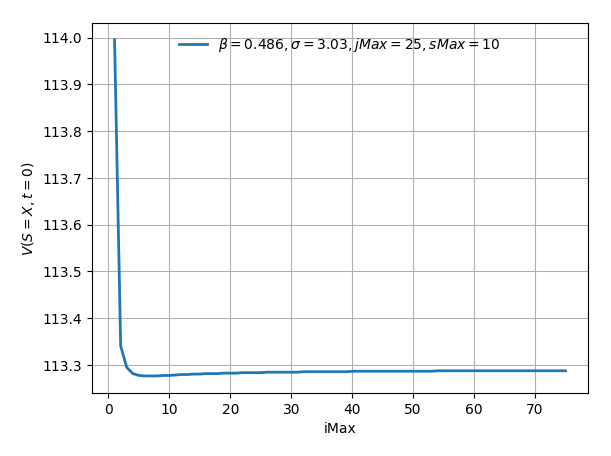
\includegraphics[width=0.5\textwidth,center]{../images/european_varying_imax.png}
\caption{Trend of the convertible bond $V(S=X,t=T)$ as parameter $i_{max}$ is varied.}
\label{fig:varying_imax}
\end{figure}
Finally, for this section the parameters $i_{max}$, $j_{max}$ and $S_{max}$ were investigated to study how a variation in their value affected the result.
The region selected was the at-the-money $S=X$ region of stock price to have comparable results across all three parameters.
Starting with the variation in the time steps, Figure \ref{fig:varying_imax} illustrates such relationship.
Here, it is clear that increasing $i_{max}$ rapidly converges towards a single value of $V(X,T)$ and after $i_{max}=25$ there is really no point in increasing this parameter too much.
\begin{figure}[!b]
\centering
\begin{minipage}{.55\textwidth}
  \centering
  \begin{subfigure}{\textwidth}
      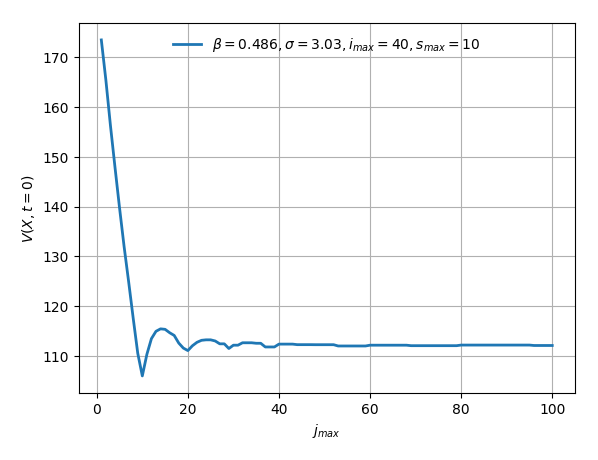
\includegraphics[width=\linewidth]{../images/smax_jmax/10_european_varying_jmax.png}
      \subcaption{Stability and convergence can be obverved after $j_{max}=40$}

  \end{subfigure}
  \label{fig:varying_jmax_10}
\end{minipage}
\end{figure}
\medskip
\begin{figure}[!ht]\ContinuedFloat
\centering
\begin{minipage}{.55\textwidth}
  \centering
  \begin{subfigure}{\textwidth}
      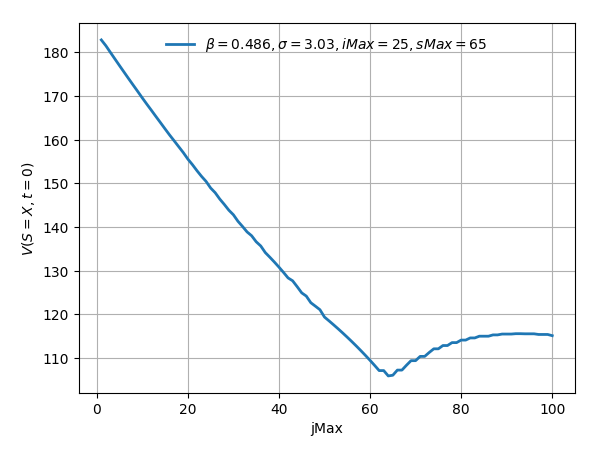
\includegraphics[width=\linewidth]{../images/smax_jmax/65_european_varying_jmax.png}
      \subcaption{The plot from \ref{fig:varying_jmax_10} is stretched and since $S_{max}$ is x6.5 as much, the first minimum is also stretched by that much.}
      \label{fig:varying_jmax_65}
  \end{subfigure}
\end{minipage}
\caption{Plots of the price of the convertible bond $V(X,T)$ against changing $j_{max}$ for different values of $S_{max}$.}
\label{fig:varying_jmax}
\end{figure}
\\
\\
When it came to varying $j_{max}$ which is the number of steps in $S$ per timestep, it was noticed
that since the stepsize in $S$ is calculated by dividing $S_{max}$ by the number of steps then these had to go
hand in hand when varying one of them.
Figure \ref{fig:varying_jmax} illustrates this very clearly.
Keeping the range of $j_{max}$ the same and increasing $S_{max}$ shows the same plot but being stretched out in the x-axis.
This happens since increasing the maximum cutoff $S$ from which to start at each timestep but keeping the number of steps constant would mean larger jumps
thus a less accurate result everytime.
Instead, ensuring that the overally stepsize in $S$ is constant or small enough is paramount in keeping the result accurate.
Recall that the error in the Crank-Nicolson method is $\mathcal{O}({\Delta S}^2,{\Delta t}^2)$.
\\
\par
Following this, the natural progression is to vary $S_{max}$ for a given value of $i_{max}.$
However, due to the results in Figure \ref{fig:varying_jmax} we have to make sure we increase $j_{max}$ as we go along.
\begin{figure}[!h]
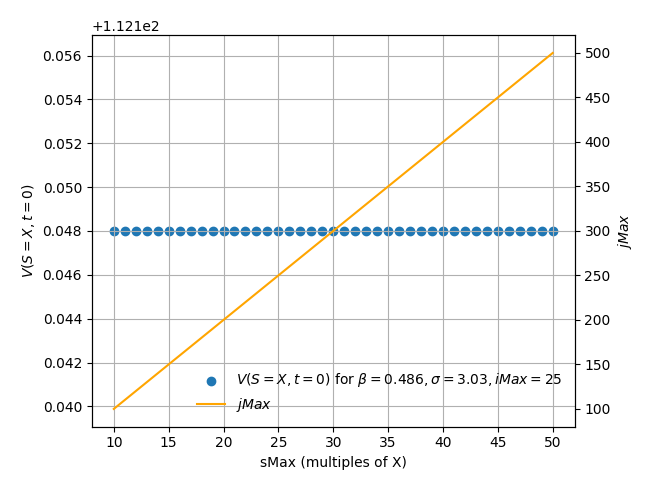
\includegraphics[width=0.65\textwidth,center]{../images/european_varying_smax.png}
\caption{Trend of the convertible bond $V(S=X,t=0)$ as parameter $S_{max}$ is varied and $j_{max}$ is varied to be kept at a comparable value.}
\label{fig:varying_smax}
\end{figure}
Figure \ref{fig:varying_smax} clearly shows that already at $S_{max}=10X$ the value of the convertible bond converges.
In fact, for higher $S_{max}$ the result is identical to 7 significant figures since this is the residual error limit that was set on the SOR method, with a maximum cap of 10,000 iterations which all iterations of $S_{max}$ shown stay under.
The computational requirement of increasing $S_{max}$ is linked to that of increasing $j_{max}$ and since the return is an unreasonable amount of significant figures precision then it is not worth using an $S_{max}>10X$.
\\
\par
The last issue left to investigate is the time requirements and processing complexity of varying these parameters.
As can be infered from Figure \ref{fig:varying_smax} $i_max$ follows a linear time increase while $j_max$ is exponential.
This is because of the fact that a single loop from time $t=T$ to $t=0$ is done but a further loop of $j_{max}$ length is done per time step.
Since the error of Crank-Nicolson is given by $\mathcal{O}({\Delta S}^2,{\Delta t}^2)$ both quantities are important and are dependent directly on $i_{max}$ and $j_{max}$ however $j_{max}$ has the highest influence on the value converging to the analytic value so a compromise must be made.
\begin{figure}[!h]
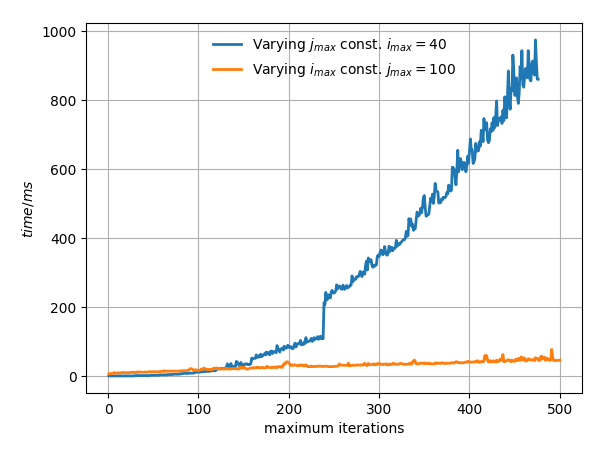
\includegraphics[width=0.65\textwidth,center]{../images/european_time.png}
\caption{Variation of the time required to calculate the convertible bond price as $j_{max}$ and $i_{max}$ are varied.}
\label{fig:varying_smax}
\end{figure}
\\
The final value for $\sigma=3.03$ and $\beta=0.486$ was calculated to be $V(S=X,t=0)=112.163$ with $S_{max}=10X$, $j_{max}=400$, $i_{max}=50$.
\clearpage
\bibliography{references}
\bibliographystyle{ieeetr}
\clearpage
\section*{Appendix 2}
\lstset{style=mystyle}
\subsection*{Portfolio Pricing Program Listing}
\lstinputlisting[language=C++]{../assignment_4.cpp}
\subsection*{Graphing Program Listing}
\lstinputlisting[language=Python]{../analytic.py}
\lstinputlisting[language=Python]{../assignment_4.py}
\end{document}